\newpage
\section{2D OFET simulations}
\label{sec:ofet}

\begin{figure}[H]

\begin{tabular}{ c l }


\includegraphics[width=0.05\textwidth]{./images/youtube.png}

&
\href{https://www.youtube.com/watch?v=0RK9GEyb4HQ}{Tutorial on OFET simulation.}

\end{tabular}
\end{figure}

Gpvdm contains a 2D electrical solver which can be used for simulating OFETs and other 2D structures.  To perform 2D simulations use the default OFET simulation in gpvdm as a starting point.  You can do this by double clicking on \emph{OFET simulation} in the new simulation window (see figure \ref{fig:ofetnewsim}).
\\
\\
\fbox{
\parbox{0.9\textwidth}{
\color{black} Note: The 2D electrical solver is a separate plug in to the 1D solver, if you select the default OFET simulation gpvdm as a starting point for your own 2D simulations gpvdm will be all set up to do 2D electrical simulations.  If you try to convert a 1D simulation such as a solar cell to a 2D simulation (not recommended) please read section \ref{sec:solverconfig} on how to select the correct solver.
}\par
}
\\
\\




To make a new OFET simulation, click on the new simulation button. In the new simulation window and select the OFET simulation (see figure \ref{fig:ofetnewsim}).  This will bring up the initial OFET simulation shown in figure \ref{fig:ofetstartsim}.

\begin{figure}[H]
\centering
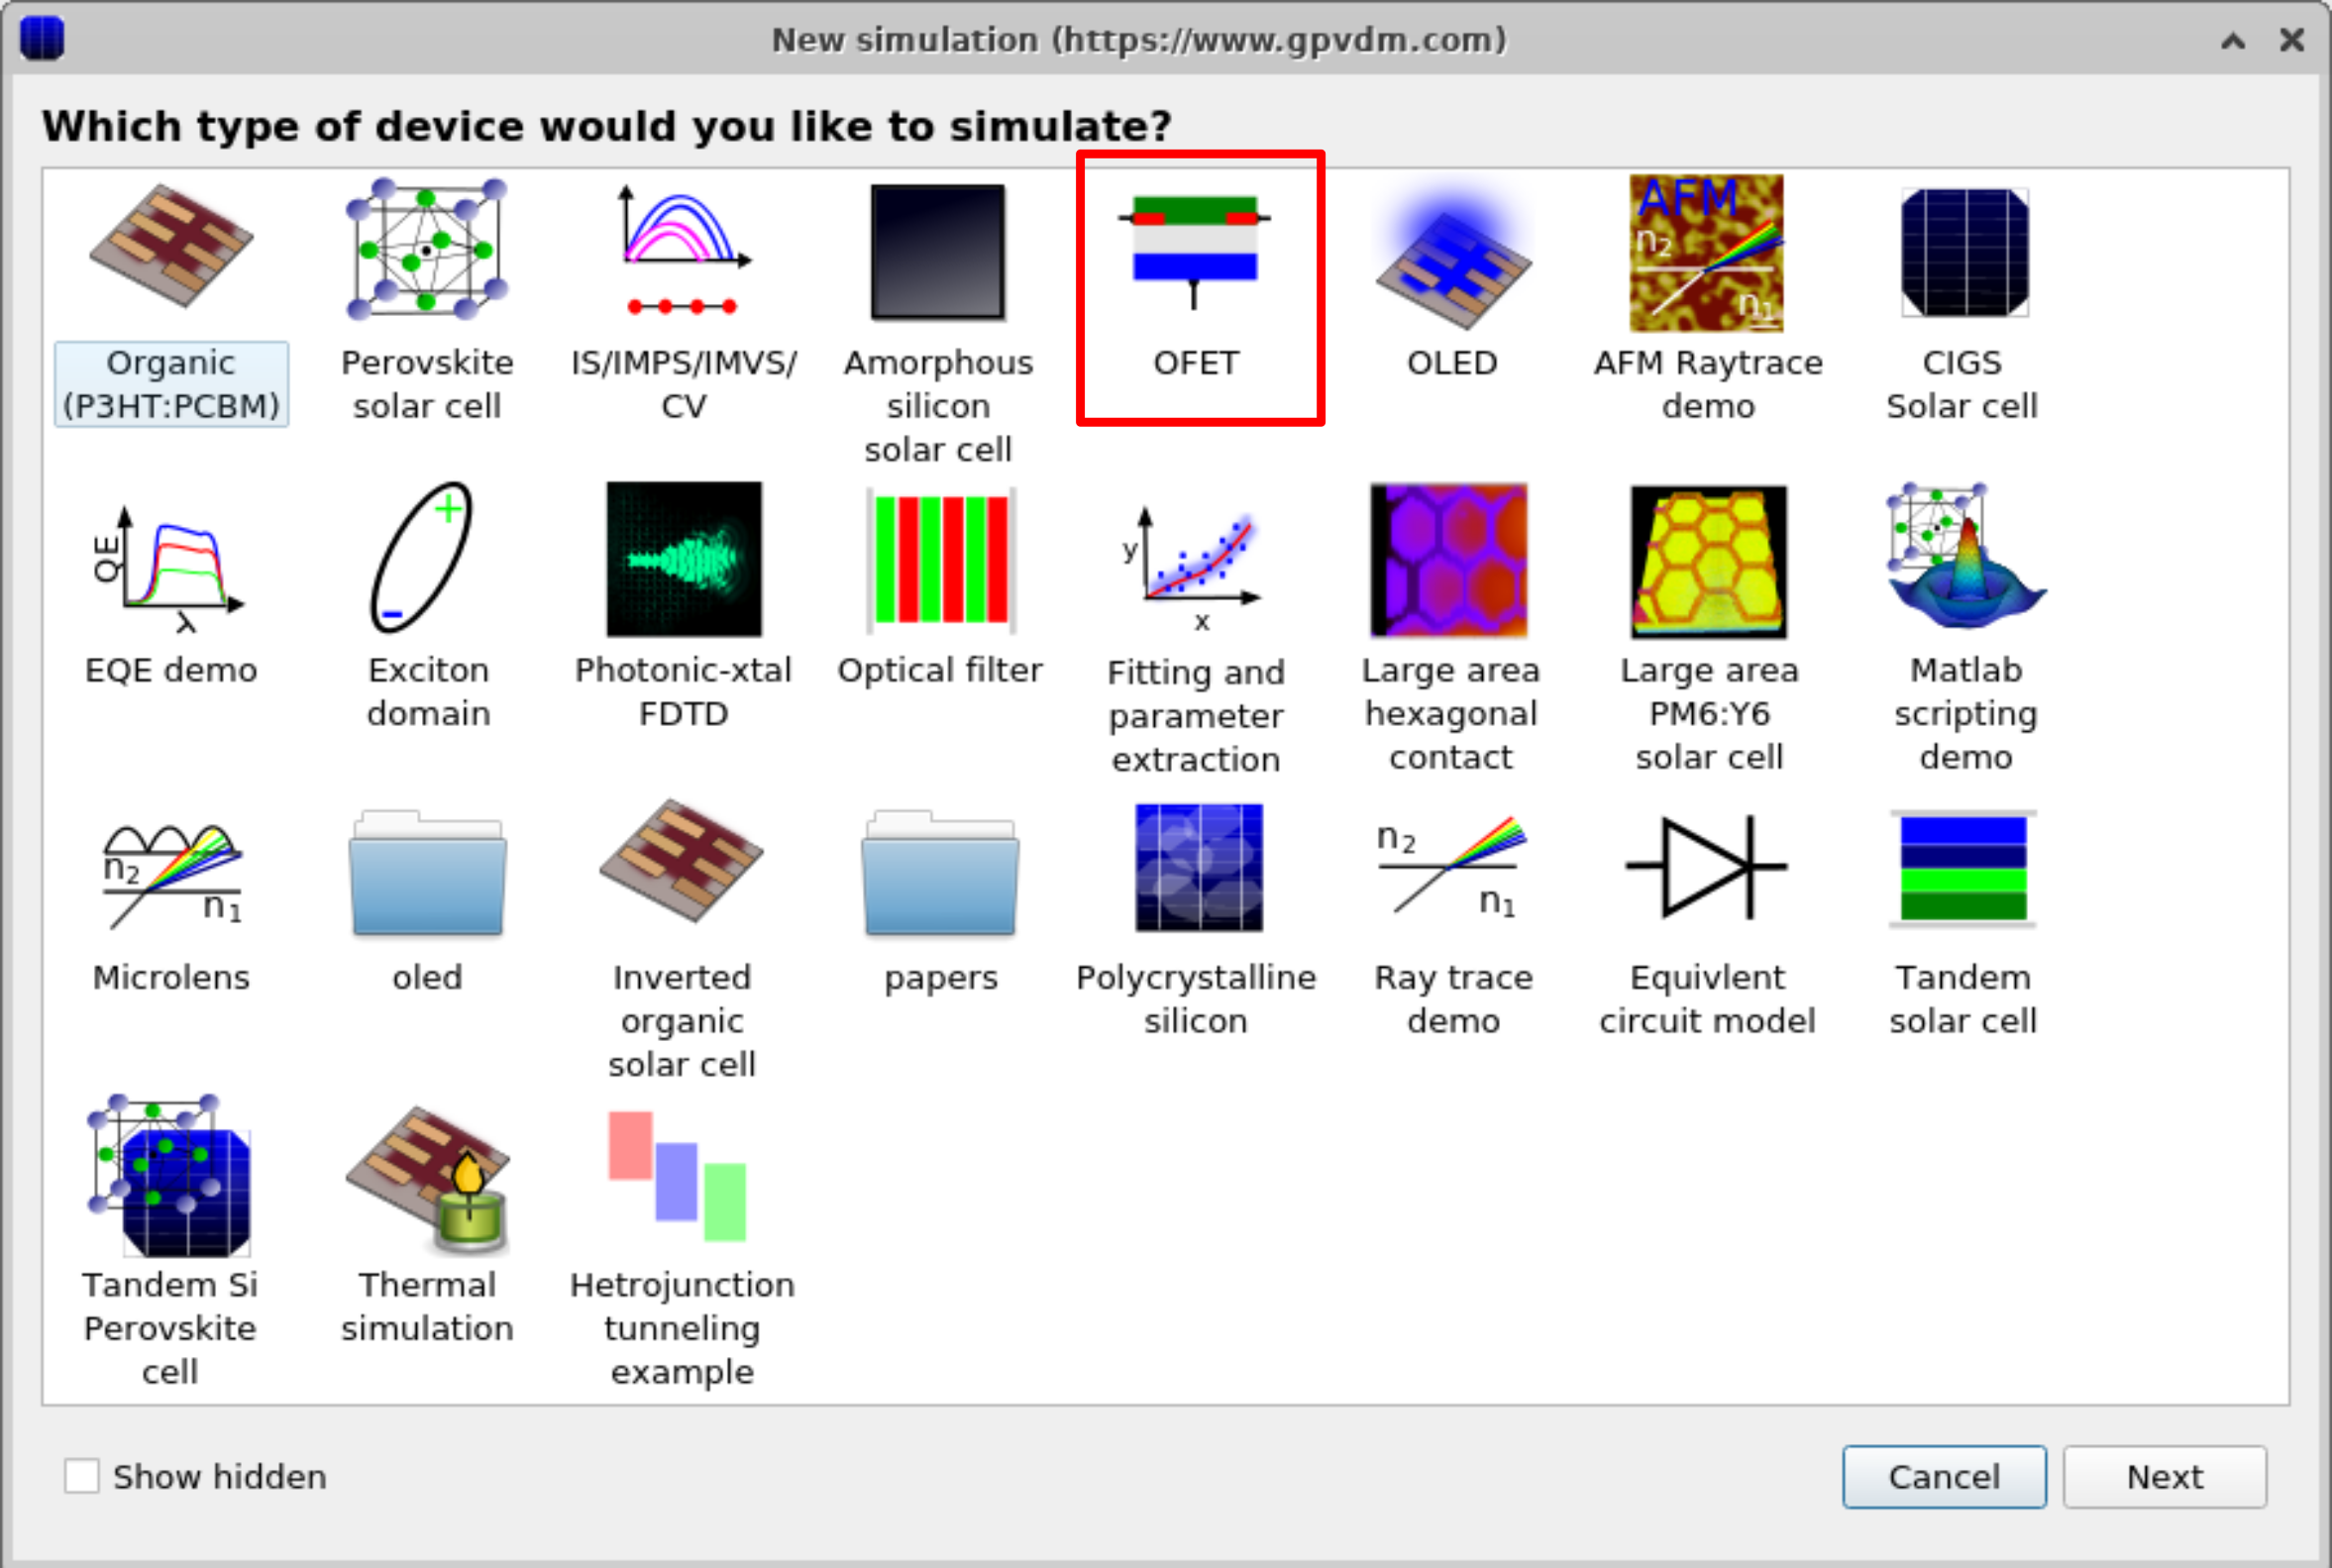
\includegraphics[width=0.7\textwidth]{./images/ofet_0.png}
\caption{Opening a new ofet simulation}
\label{fig:ofetnewsim}
\end{figure}




\subsection{The anatomy of a 2D simulation}

\begin{figure}[H]
\centering
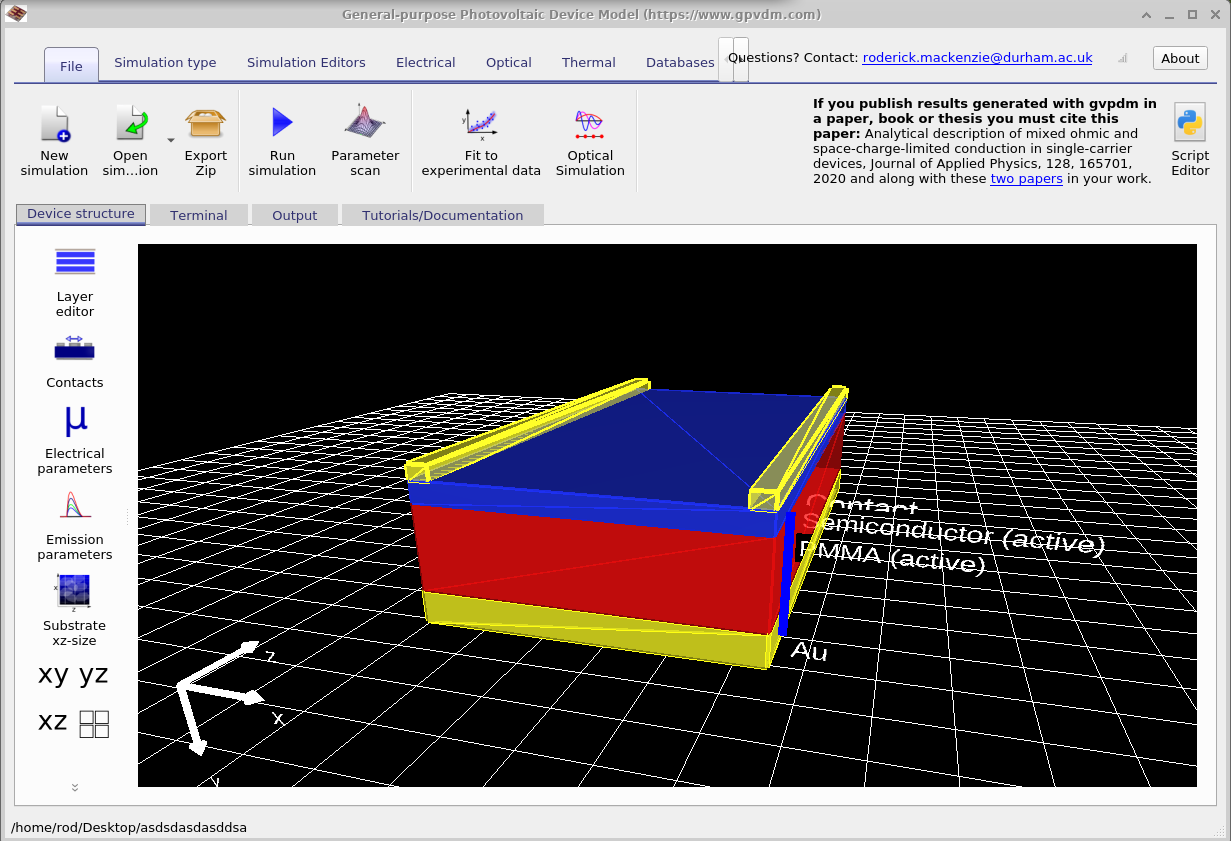
\includegraphics[width=0.7\textwidth]{./images/ofet_1.png}
\caption{The default ofet simulation.}
\label{fig:ofetstartsim}
\end{figure}

The OFET structure shown in figure \ref{fig:ofetstartsim} consists of a \emph{gate} and \emph{drain} contact shown on the top of the simulation as gold bars, a semiconductor layer is shown in blue and an insulating later shown in red.  A \emph{gate} contact is also visible at the bottom of the structure.  This layer structure is defined in layer editor, see figure \ref{fig:ofetlayerstructure}. The layer editor has been described in detail in section \ref{sec:layereditor}. It can be seen that the top and bottom layers have been set to \emph{contact} and the insulator (PMMA) and semiconducting layer have been set to active. This means that the drift diffusion equations will be solved over the semiconductor and insulator layers and the contacts will be used as boundary conditions.  As this structure is not emitting light the \emph{Optical material} column has no impact on the simulation results.

%\fbox{
%\parbox{0.9\textwidth}{
%\color{blue} Task \addtocounter{question}{1}\thequestion : Try changing the heigh of the gate layer from 100nm to 500 nm and see what ahpp
%}\par
%}
%\\


\begin{figure}[H]
\centering
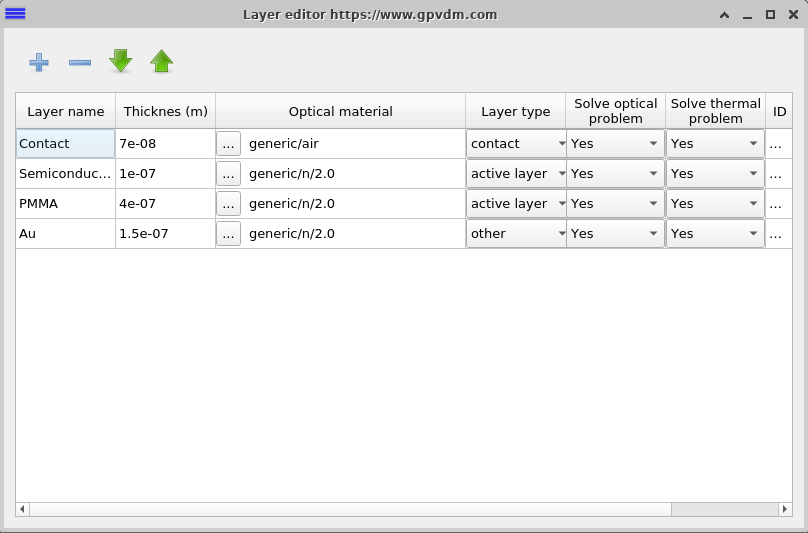
\includegraphics[width=0.7\textwidth]{./images/ofet_2.png}
\caption{The layers of an OFET device}
\label{fig:ofetlayerstructure}
\end{figure}

The contacts are defined in the contact editor shown in figure \ref{fig:ofetcontacteditor}. The contact editor has been described in detail in 
section \ref{sec:contacteditor}, however because this is a 2D simulation another two extra columns have appeared. They are \emph{start} and \emph{width}.  These define the start position of the contact on the x-axis and width which describes the width of the contact on the x-axis.  The \emph{source} starts at $0~m$ and extends to $5 \mu m$, the  \emph{drain} starts at $75~\mu m$ and extends to $5 \mu m$, while the gate starts at $0~m$ and extends to cover the entire width of the device which is $80~ \mu m$.  If you are unsure which is the x-axis, the origin marker is visible at the bottom of figure \ref{fig:ofetstartsim}.

\begin{figure}[H]
\centering
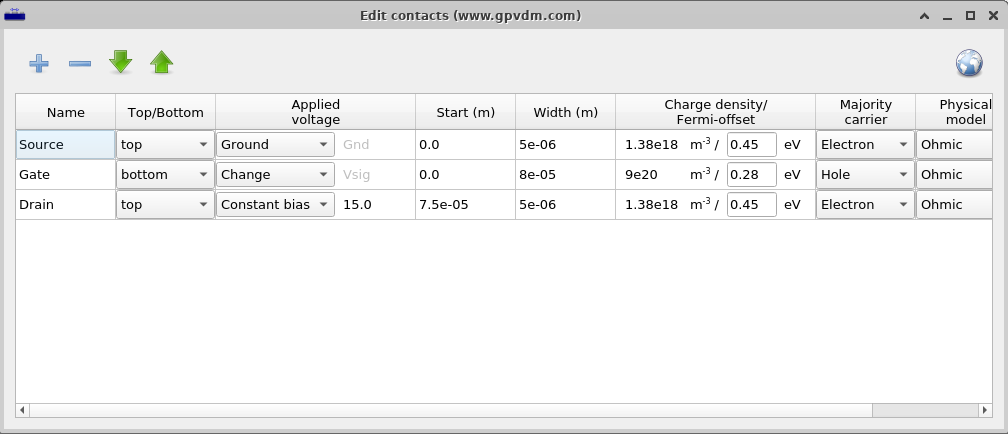
\includegraphics[width=0.7\textwidth]{./images/ofet_3.png}
\caption{Editing the contacts on a 2D device.}
\label{fig:ofetcontacteditor}
\end{figure}

The electrical parameters for both the semiconductor and the insulator can be seen in figure \ref{fig:ofetelectricalparamters}, these can be accessed through the \emph{Electrical parameter} editor. The \emph{Electrical parameter} editor is described in detail in section \ref{sec:doseditor}. To the left of the figure the parameters for the semiconducting layer are described and to the right of the figure the parameters for the insulating layer are described. Below I have made comments on each parameter in relation to OFET simulation.

\begin{itemize}
  \item Mobility: The free carrier mobility in the active layer will be defined by the semiconductor you are trying to simulate.  The mobility in the insulator is usually set to a low value such as $1e-12-1e-15$ to limit current flow into the region. However, the value should not be set too low (see section \ref{sec:solverstability}) or the solver may become numerically unstable.
  \item Effective density of states: Keep these the same for both layers, just to keep things simple.
  \item Number of trap states: You can set this to what value you want to but if you choose a large number in 2D it will significantly affect the speed of the simulation, simply because \emph{number of equation solved=XMESHPOINTS $\times$ YMESHPOINTS $\times$ NUMEROFTRAPS}.
  \item Eg and Xi: Although it is tempting to simply enter the experimental values for Xi and Eg for both the insulator and the semiconductor, one has to be careful in doing this as some insulators ($SiO_2$) have very big band gaps which mean the number of carriers get very small and make the simulation unstable (read section \ref{sec:solverstability} for an explanation).  If you want to simulate a jump in the band gap into an insulator, my is to make the jump significantly bigger than $3/2kT=25meV$ which is the average kinetic energy of a charge carrier.  If the gap is between $0.5-1.0 V$ charge carriers will have problems penetrating the barrier and there is no need to simulate bigger steps.
\end{itemize}

\begin{figure}[H]
\centering
\begin{tabular}{ c c }

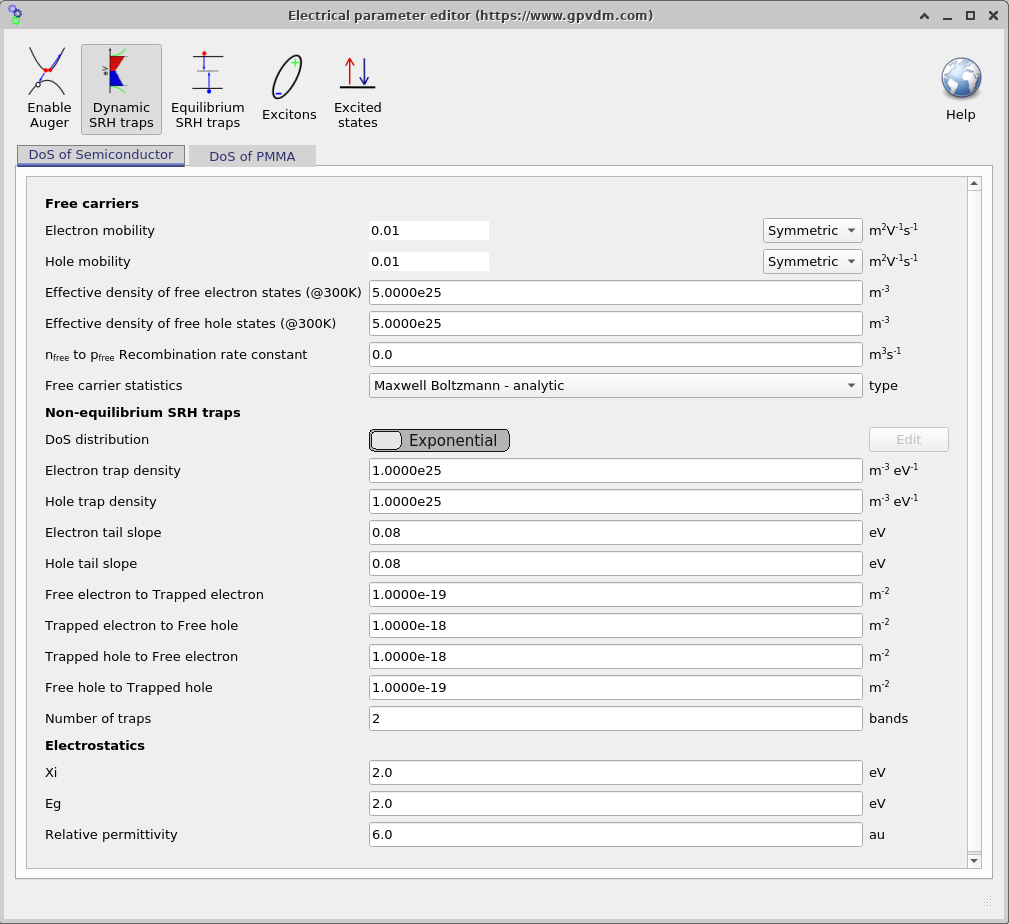
\includegraphics[width=0.5\textwidth,height=0.4\textwidth]{./images/ofet_5.png}

&
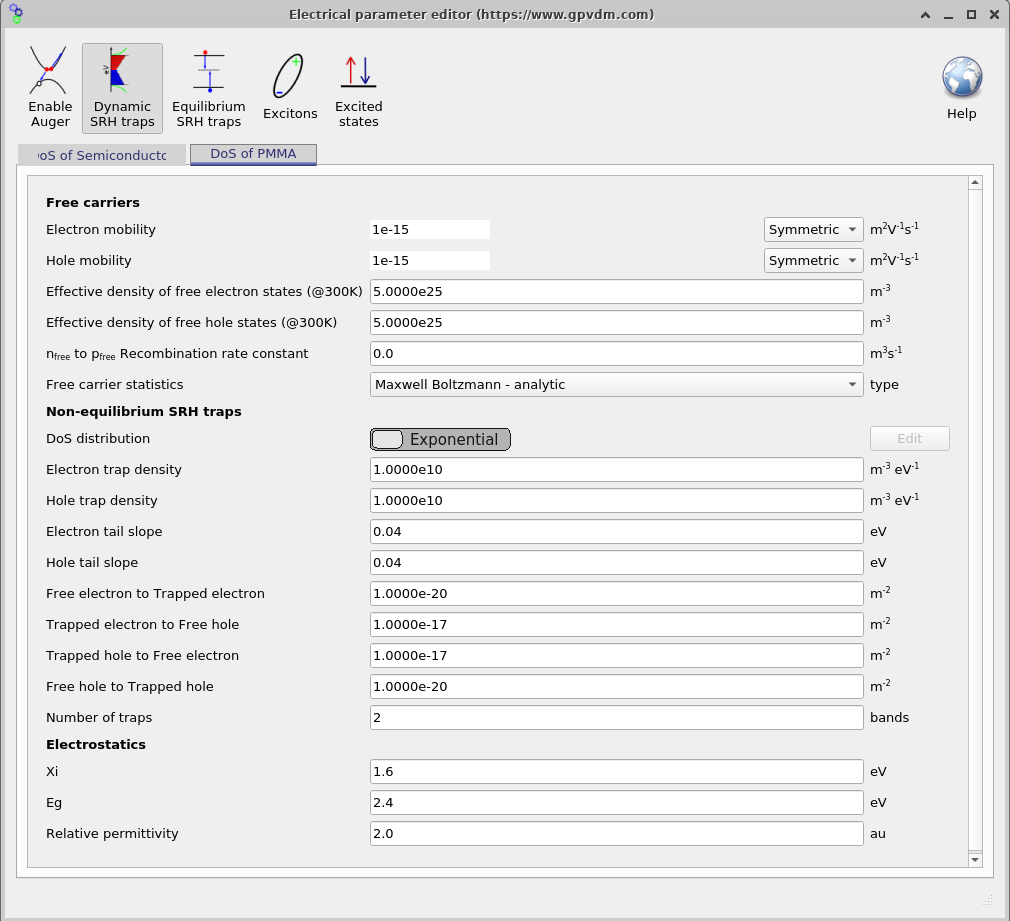
\includegraphics[width=0.5\textwidth,height=0.4\textwidth]{./images/ofet_6.png}
\\
\end{tabular}
\caption{Electrical parameters for both the semiconductor (left) and the insulator (right)}
\label{fig:ofetelectricalparamters}
\end{figure}

\subsection{Running a 2D simulation}

2D simulations are run in the same way as 1D simulations, simply click on the play button, see figure \ref{fig:ofetrun}.
\begin{figure}[H]
\centering
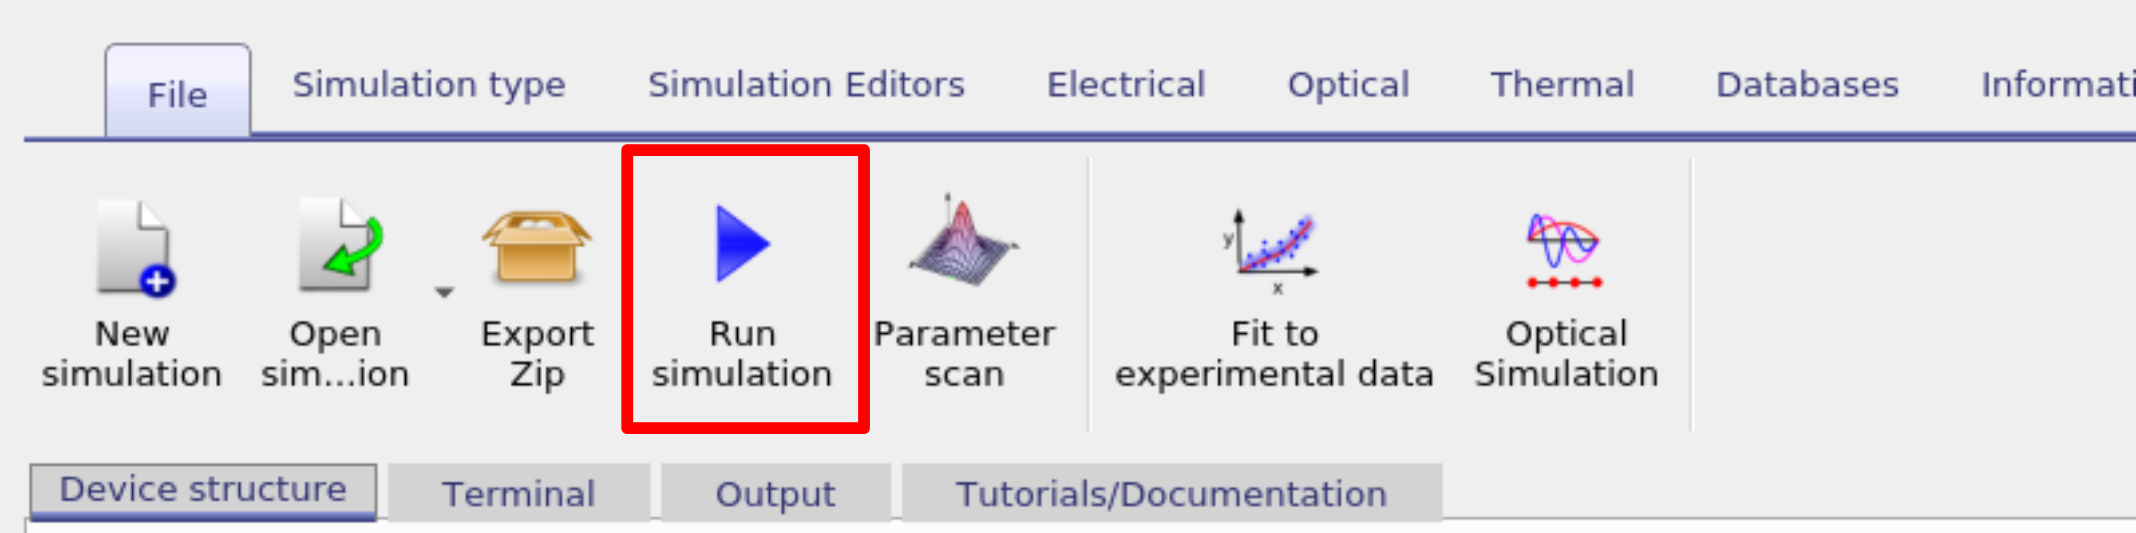
\includegraphics[width=0.7\textwidth]{./images/run_sim.png}
\caption{Running an OFET simulation}
\label{fig:ofetrun}
\end{figure}

The simulation will take longer than it's 1D counterparts simply because there will be more equations to solve.  If you have set a contact at a high starting voltage the solver will initially ramp the contact voltage in a stepwise way until the desired voltage is achieved before the desired voltage sweep is applied to the \emph{active contact}. After the simulation has run the following files will be produced showing the current density from each contact.


\begin{itemize}
  \item contact\textunderscore iv0.dat:
  \item contact\textunderscore iv1.dat:
  \item contact\textunderscore iv2.dat:

  \item contact\textunderscore jv0.dat:
  \item contact\textunderscore jv1.dat:
  \item contact\textunderscore jv2.dat:

  \item snapshots:

\end{itemize}

\begin{figure}[H]
\centering
\begin{tabular}{ c c }

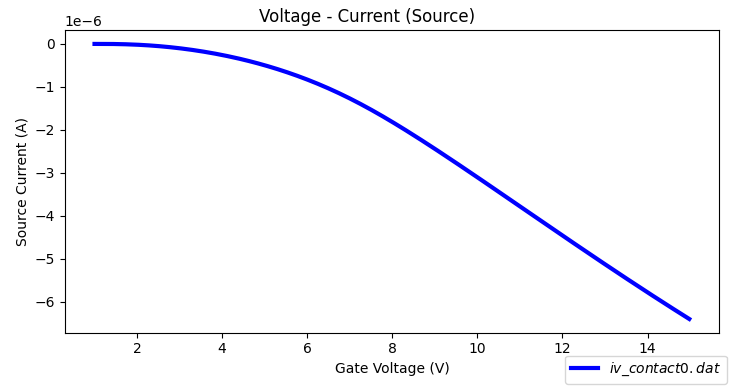
\includegraphics[width=0.5\textwidth,height=0.4\textwidth]{./images/ofet_7.png}

&
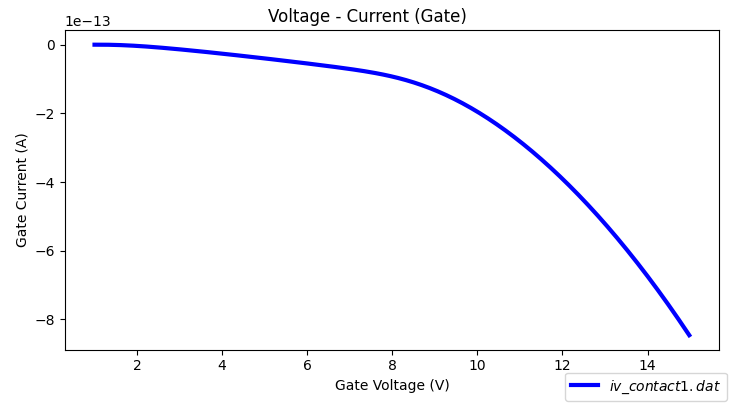
\includegraphics[width=0.5\textwidth,height=0.4\textwidth]{./images/ofet_8.png}
\\

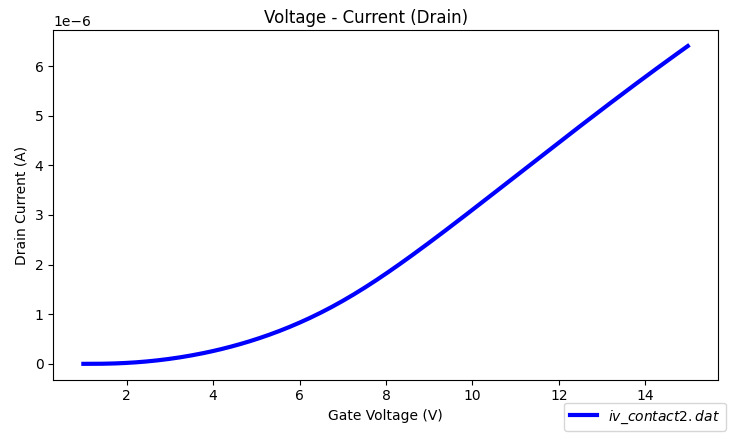
\includegraphics[width=0.5\textwidth,height=0.4\textwidth]{./images/ofet_9.png}

&
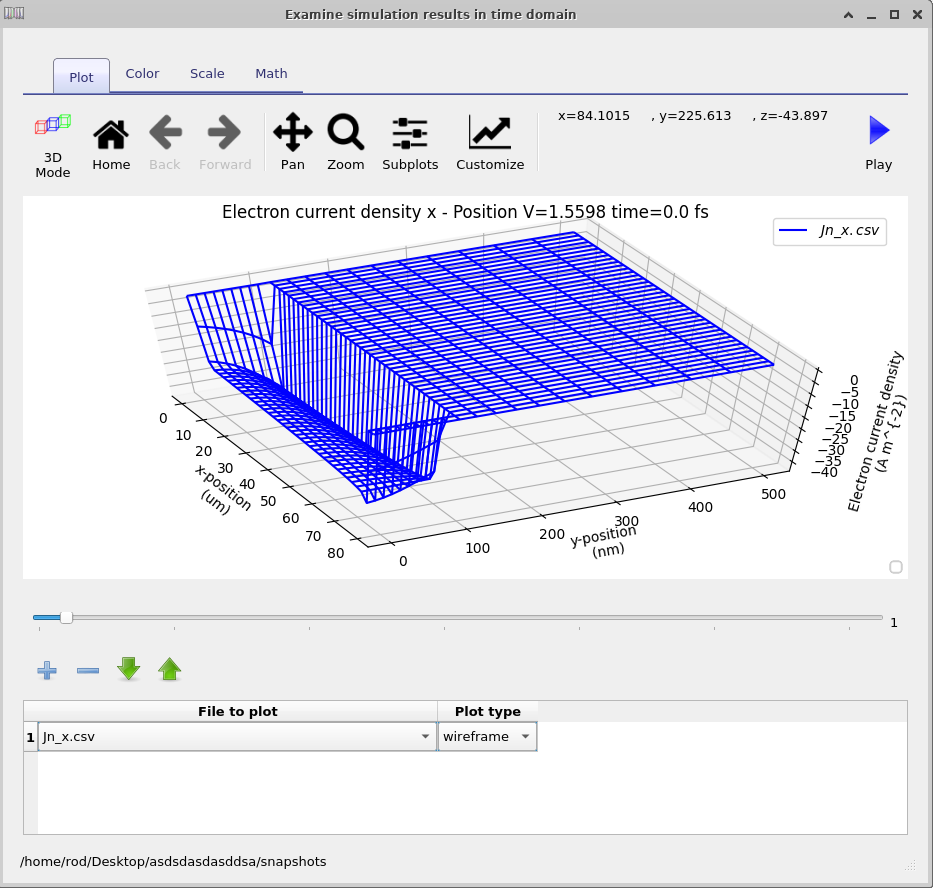
\includegraphics[width=0.5\textwidth,height=0.4\textwidth]{./images/ofet_10.png}
\\
\end{tabular}
\caption{Electrical parameters}
\end{figure}

\subsection{Meshing in 2D}

\begin{figure}[H]
\centering
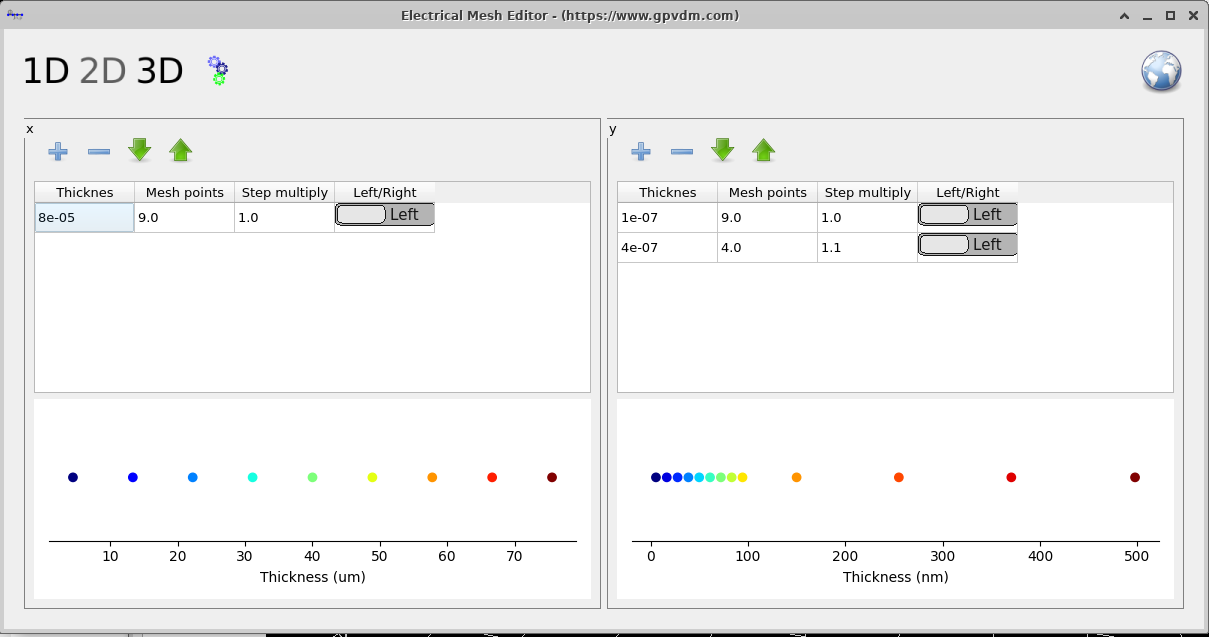
\includegraphics[width=0.7\textwidth]{./images/ofet_4.png}
\caption{Meshing}
\label{fig:ofetmeshing}
\end{figure}









